%%=============================================================================
%% Opstellen ontwikkelomgeving
%%=============================================================================

\chapter{Opstellen ontwikkelomgeving}%
\label{ch:ontwikkelomgeving}

Vooraleer het onderzoek van start kan, moet de ontwikkelomgeving voor zowel native 
als cross-platform opgesteld worden. 
\\\\
Zoals besproken in hoofdstuk \ref{ch:stand-van-zaken} zullen we voor native ontwikkeling Kotlin 
met Android Studio gebruiken om applicaties te ontwikkelen. Voor cross-platform zullen we React Native 
met Visual Studio Code gebruiken.

\section{Opstellen native ontwikkeling}\label{se:native}

Om met native ontwikkeling van start te gaan zullen we eerst Android Studio moeten downloaden. 
Dit kan vanop de website \url{https://developer.android.com/studio/}

\paragraph{1. Components}
Bij het eerste scherm van het installatieprogramma is het belangrijk om ook 
\textbf{Android Virtual Device} te selecteren. Deze stelt ons in staat om de applicaties die we 
zowel voor native als cross-platform zullen ontwikkelen kunnen runnen. 

\paragraph{2. Installatie locatie}
Op het volgend scherm kiezen we de locatie waar Android Studio geïnstalleerd wordt. 
Het is aangeraden om dit niet te vervangen omdat React native gebruik maakt van de standaard 
locatie om bepaalde componenten op te zoeken. 

\paragraph{3. Startmenu map}
Deze is zelf te kiezen. Hiermee creëer je een shortcut vanwaar Android Studio kan worden opgestart.

\paragraph{4. Android SDK}\label{par:sdk}
Als de installatie goed is verlopen krijgen we volgend welkom scherm te zien. 
\begin{figure}[H]
    \centering
    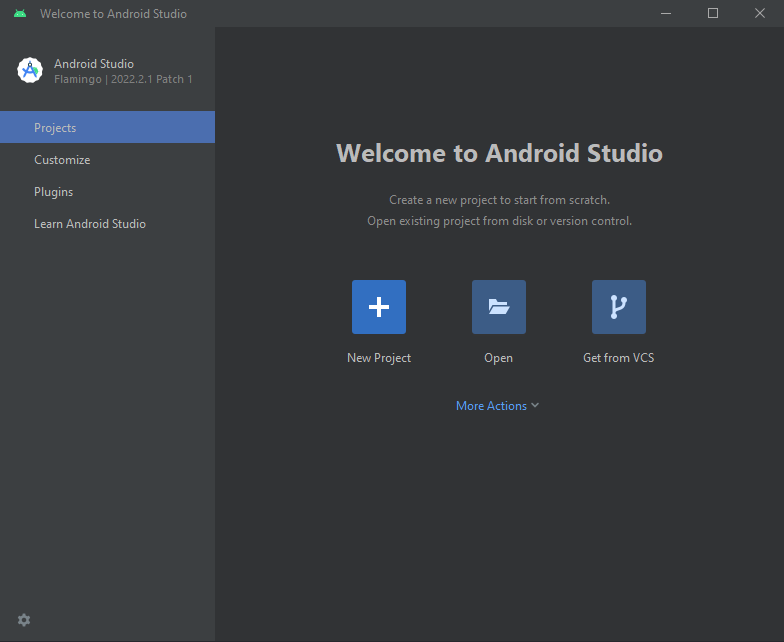
\includegraphics[height=0.4\textheight]{androidinstallatie.png}
    \caption{Startscherm na Android Studio installatie.}
\end{figure}
Standaard wordt de laatste Android SDK geïnstalleerd door Android Studio. 
Deze zullen we ook tijdens de duratie van het onderzoek gebruiken. 
Maar om met deze laatste Android SDK te werken hebben we Android 13 (Tiramisu) nodig. 
Om deze te installeren drukken we op \textit{More Actions}. Op het nieuwe verkregen scherm 
kunnen we dan Android 13 (Tiramisu) aanvinken. Ook zullen we onderaan rechts het vakje 
\textbf{Show Package Details} aanvinken om dan te verifiëren dat ook zeker 
\textbf{Android SDK Platform 33}, \textbf{Sources for Android 33} en 
\textbf{Google APIs Intel x86\_64 Atom System Image} zijn aangevinkt.
\\\\
Daarna navigeren we naar SDK Tools en vinken we opnieuw \textbf{Show Package Details} 
aan en vinken we ook onder Android SDK Build-Tools \textbf{33.0.0} aan. 
Tot slot drukken we op \textbf{Apply} om de Android SDK en gerelateerde tools te downloaden en installeren. 
Maak daarna ook een dummy project aan (Empty Activity) om Android Studio van start te krijgen.

\paragraph{5. Emulator}
Om de applicaties die we zullen ontwikkelen te runnen hebben we een emulator nodig. 
Deze kunnen we aanmaken bovenaan rechts \textit{Device Manager > Create device}. 
Eerst en vooral selecteren we de device dat we willen emuleren. Voor het onderzoek 
gaan we gebruik maken van een Pixel 3 als device. Na het selecteren van ons device moeten we 
de Android versie klikken. Hier selecteren we Tiramisu met API Level 33 (Die we daarnet hebben geïnstalleerd). 
Tot slot zijn er nog een aantal configuratie instellingen voor het apparaat. Wij laten deze allemaal op hun standaard 
waarden staan.
\\\\
Nu is Android Studio klaar om native applicaties te ontwikkelen en runnen. 


\section{Opstellen cross-platform ontwikkeling}

Om cross-platform te ontwikkelen door gebruik te maken van React native is er wat meer werk om 
de omgeving op te stellen. Eerst zullen we Visual Studio Code downloaden. 
Dit kan vanop de website \url{https://code.visualstudio.com/download} 

Na het installeren van Visual Studio Code kunnen we de React native ontwikkelomgeving opstellen. 
Dit kan door de handleiding te volgen vanop de website \url{https://reactnative.dev/docs/environment-setup}.

\paragraph{1. React Native CLI Quickstart}
Voor de React native ontwikkelomgeving kunnen we ook gebruik maken van Expo. 
Dit is een simpele manier om snel applicaties visueel werkend te krijgen. 
Maar voor dit onderzoek zullen we de applicaties op dezelfde emulator runnen waarop de native 
ontwikkelde applicaties runnen. Hiervoor volgen we de React Native CLI Quickstart handleiding. 

\paragraph{2. Besturingssysteem en doelsysteem}
Afhankelijk van het gebruikte besturingssysteem is er een andere handleiding. 
Doorheen dit onderzoek zullen we werken op een Windows laptop en zullen we focussen op Android applicaties.

\paragraph{3. Node \& JDK}
Als eerste moeten we \Gls{Node} en \acrshort{jdk} installeren. Dit kunnen we makkelijk 
doen met \Gls{Chocolatey}. Chocolatey indien niet geïnstalleerd kan worden gedownload 
vanop de website \url{https://chocolatey.org/install}. Eerst openen we een 
opdrachtprompt (powershell) als administrator waaraan we volgende commando meegeven.
\begin{minted}{bash}
choco install -y nodejs-lts microsoft-openjdk11
\end{minted}
Voor Node gebruiken we de laatste versie. De minimale versie waarmee React native kan werken is 14. 
Voor de JDK gebruiken we versie 11 aangezien hogere versies voor problemen kunnen zorgen.

\paragraph{4. Android ontwikkelomgeving}
Net zoals bij native ontwikkeling hebben we voor React native applicaties ook Android Studio nodig. 
Dit is omdat we om de applicatie te runnen gebruik maken van de emulator binnenin Android Studio. 
Android Studio zelf wordt niet direct gebruikt maar er wordt enkel gebruik gemaakt van de 
emulator die Android Studio aanbied.
\\\\
Bij het opstellen van de React native omgeving zijn er een paar instellingen waar we rekening 
mee moeten houden. Maar hiermee is al rekening gehouden bij het installeren van Android Studio 
in paragraaf \ref{par:sdk}.

\paragraph{5. ANDROID\_HOME omgevingsvariabelen}
De React native tools hebben enkele omgevingsvariabelen nodig om native applicaties te bouwen. 
Om deze omgevingsvariabelen in te stellen openen we eerst het configuratiescherm van Windows. 
Daarna gaan we naar 
\textit{Gebruikersaccounts > Gebruikersaccounts > Mijn omgevingsvariabelen veranderen > Nieuw\dots}. 
In het nieuwe verkregen scherm vullen we dan de naam van de omgevingsvariabel \textbf{ANDROID\_HOME} 
en de path naar de Android SDK in. De standaard path naar de Android SDK is 
\textbf{\%LOCALAPPDATA\%\backslash Android\backslash Sdk}. 
De locatie van de Android SDK is ook te vinden via Android Studio via 
\textit{File > Settings > Appearance \& Behavior > System Settings > Android SDK}.
\\\\
Om te controleren dat de omgevingsvariabel correct is toegevoegd openen we een nieuwe 
opdrachtprompt (powershell) en geven we volgend commando in.
\begin{minted}{bash}
Get-ChildItem -Path Env:\
\end{minted}
In de teruggegeven lijst controleren we dan of dat ANDROID\_HOME effectief is toegevoegd.
\\\\
Tot slot moeten we de \textbf{Path} omgevingsvariabel aanpassen. 
Opnieuw navigeren we in het configuratiescherm naar het overzicht met alle omgevingsvariabelen 
\textit{Gebruikersaccounts > Gebruikersaccounts > Mijn omgevingsvariabelen veranderen}. 
Hierin selecteren we de Path omgevingsvariabel en daarna drukken we op \textit{Bewerken...}. 
Bij het nieuw verkregen scherm drukken we op \textit{Nieuw} en voegen we de path naar platform-tools 
toe aan de lijst. Het path van de platform-tool is standaard 
\textbf{\%LOCALAPPDATA\%\backslash Android\backslash Sdk\backslash platform-tools}.

\paragraph{6. React native Command Lin Interface (CLI)}
React native heeft een ingebouwde command line interface (CLI) om te werken met React native. 
Deze kan gebruikt worden dankzij Node.js dat we daarnet installeerden.
\begin{minted}{bash}
npx react native [commando]
\end{minted}

\paragraph{7. Emulator gebruiken} \label{par:emulatorgebruiken}
Om nu effectief applicaties te laten runnen maken we gebruik van de emulator die Android Studio aanbied. 
Aangezien deze al opgesteld is bij het opzetten van Android Studio \ref{se:native} 
moeten we dit niet meer doen voor React native. Om de applicatie starten hebben we twee terminals nodig 
binnen Visual Studio code, deze kunnen we openen via \textit{Terminal > New Terminal}. 
In de eerste terminal starten we \Gls{Metro} met het volgende commando.
\begin{minted}{bash}
npx react-native start
\end{minted}
In de tweede terminal geven we het volgende commando dat de applicatie zal opbouwen en 
deployen naar de emulator.
\begin{minted}{bash}
npx react-native run-android
\end{minted}

\section{Gebruikte hardware tijdens onderzoek}

Doorheen het onderzoek zullen alle projecten starten vanuit een blanco project en op dezelfde emulator 
getest worden. Deze emulator zal altijd runnen op hetzelfde apparaat. Dankzij volgend commando 
kunnen we de informatie verkrijgen van een apparaat:
\begin{minted}{bash}
npx react-native info
\end{minted}
Deze geeft bij het gebruikte apparaat voor dit onderzoek volgende output:
\begin{minted}{bash}
System:
    OS: Windows 10 10.0.19044
    CPU: (12) x64 AMD Ryzen 5 5600H with Radeon Graphics
    Memory: 2.90 GB / 15.86 GB
Binaries:
    Node: 18.16.0 - C:\Program Files\nodejs\node.EXE
    Yarn: Not Found
    npm: 9.5.1 - C:\Program Files\nodejs\npm.CMD
    Watchman: Not Found
SDKs:
    Android SDK: Not Found
    Windows SDK: Not Found
IDEs:
    Android Studio: AI-222.4459.24.2221.9971841
    Visual Studio: Not Found
Languages:
    Java: 11.0.18
npmPackages:
    @react-native-community/cli: Not Found
    react: 18.2.0 => 18.2.0 
    react-native: 0.71.7 => 0.71.7 
    react-native-windows: Not Found
    npmGlobalPackages:
    *react-native*: Not Found
\end{minted}
Voor dit onderzoek wordt een apparaat met een AMD Ryzen 5 5600H processor 
met 12 cores, geïntegreerde Radeon Graphics en 16GB RAM geheugen gebruikt, wat sterk en snel 
genoeg is om het onderzoek uit te voeren.










